\documentclass{homework}
\usepackage{xcolor}
\usepackage{nicematrix}
\usepackage{booktabs}
\usepackage{enumitem}
\usepackage{caption}
\usepackage{float}
\usepackage{placeins}
\usepackage{subcaption}
\usepackage{graphicx}

\NiceMatrixOptions{cell-space-limits = 1pt}

\title{Solutions worksheet 02}
\author{
  Maksimov, Dmitrii\\
  \texttt{dmitrii.maksimov@fau.de}
  \and
  Ilia, Dudnik\\
  \texttt{ilia.dudnik@fau.de}
  \and
  Isa, Baghirov\\
  \texttt{isa.baghirov@fau.de}
  \and
  Yulia, Herasymenko\\
  \texttt{yuliia.herasymenko@fau.de}
}
\begin{document}

\maketitle

\exercise[{[Analytically calculating eigenvalues and eigenvectors]}]
Let $A \in \R^{n\times n}$ be a quadratic matrix. Whenever for a vector $v \in \R^n$ and for a $\lambda \in \R$ the equation
\begin{equation} \label{eq:1}
Av = \lambda v
\end{equation}
holds, we call $\lambda$ and eigenvalue of \emph{A} and \emph{v} the corresponding eigenvector. Find out how to calculate eigenvalues and eigenvectors analytically and calculate the eigenvalues and eigenvectors of the matrix
$$
A\coloneqq \frac{1}{3}\cdot \begin{pNiceMatrix}
5 & -2 & -3\\
-2 & 5 & 1\\
-1 & 1 & 8
\end{pNiceMatrix}.
$$

Given \ref{eq:1}, bring all to left hand side and put in an identity matrix \emph{I}:
\[v(A-\lambda I) = 0\]
If \emph{v} is non-zero then:
\begin{equation} \label{eq:2}
|A - \lambda I|=0
\end{equation}

\begin{align*}
|A - \lambda I| &\coloneqq (\frac{1}{3})^3\cdot 
\begin{vNiceMatrix}
5 - 3\lambda & -2 & -3\\
-2 & 5 - 3\lambda & 1\\
-1 & 1 & 8 - 3\lambda
\end{vNiceMatrix}  \\
&=\frac{1}{27}(5 - 3\lambda)((5-3\lambda)(8-3\lambda) - 1) + 2(2(3\lambda - 8) + 1) - (-2 + 5 - 3\lambda) \\
&=-\frac{1}{27}\cdot \frac{1}{27}(\lambda^3 - 6\lambda^2 + 11\lambda - 6) \\
&=-\frac{1}{27}\cdot \frac{1}{27}(\lambda - 1)(\lambda - 2)(\lambda - 3)
\end{align*}
Solving \ref{eq:2}: $\lambda_1 = 1, \lambda_2 = 2, \lambda_3 = 3$.

Let us find their matching eigenvectors using \ref{eq:1}:
$$
\begin{pNiceMatrix}
5 & -2 & -3\\
-2 & 5 & 1\\
-1 & 1 & 8
\end{pNiceMatrix}
\begin{pNiceMatrix}
v_{i_1} \\
v_{i_2}\\
v_{i_3}
\end{pNiceMatrix}
= \lambda_i
\begin{pNiceMatrix}
v_{i_1} \\
v_{i_2}\\
v_{i_3}
\end{pNiceMatrix}
, \forall i \in [1, 2, 3]
$$
Hence, $v_1 = (1, 1, 0)^T, v_2 = (-1, 1, -1)^T, v_3 = (-1, 1, 2)^T$.

\exercise*[{[Definiteness of the covariance matrix]}]
Let $y^{(1)}, \dots, y^{(N)} \in \R^M$ be centered input data and let \emph{C} be the respective covariance matrix.
\begin{enumerate}
	\item Show that \emph{C} is always positive semi-definite.

	If \emph{C} is  positive semi-definite matrix then $x^TCx \geq 0, \forall x \in \R^M$.
	\begin{align*}
	\langle x,Cx\rangle&=\langle x,(\frac{1}{N}\sum_{i=1}^Ny_i y_i^T)x\rangle \\
	&=\frac{1}{N}\sum_{i=1}^N x^T y_i y_i^T x \\
	&=\frac{1}{N}\sum_{i=1}^N \langle x, y_i\rangle \langle y_i, x\rangle \\
	&=\frac{1}{N}\sum_{i=1}^N \langle x, y_i\rangle^2 \geq 0
	\end{align*}
	\item In which cases is $\langle y,Cy\rangle = 0$ for $y \in \R^M / \vec{\{0\}}$. What does that mean for the given data?
	 \[\langle y,Cy\rangle = 0 \Longleftrightarrow rank(C) < N\]
	This can be observed in 2 cases:
	\begin{itemize}
		\item $N < M$

		It means that observations less than number of features. This is common in image datasets where a feature is a pixel.
		\item $Var(feature) = 0$

		It means that there is no dispersion in some feature, i.e. a feature is constant.
	\end{itemize}
\end{enumerate}

\exercise*[{[Implementing PCA for data reduction]}]
Plot the features after applying the PCA algorithm for $k=3$ and $k=2$. What can you observe?

Honestly, we don't understand what we have to do. So, we will do following steps:
\begin{enumerate}
	\item Plot the features after applying the PCA algorithm for $k=3$, since the distributions of features don't depend on number of \emph{k}.
	\item Show how much of the variance in data is explained depending on \emph{k}
\end{enumerate}
Plot the features after applying the PCA algorithm for $k=3$.
\newpage
\begin{figure}[hbt!]
     \centering
     \begin{subfigure}[b]{0.3\textwidth}
         \centering
         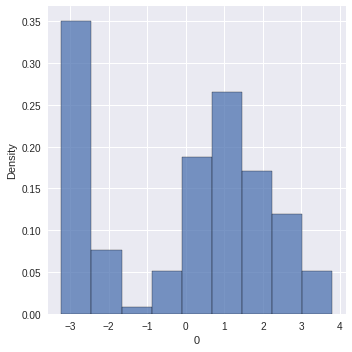
\includegraphics[width=\textwidth]{PC1_distribution.png}
         \caption{PC1}
     \end{subfigure}
     \hfill
     \begin{subfigure}[b]{0.3\textwidth}
         \centering
         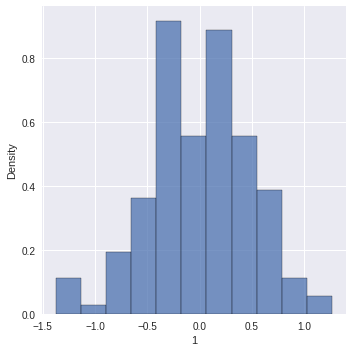
\includegraphics[width=\textwidth]{PC2_distribution.png}
         \caption{PC2}
     \end{subfigure}
     \hfill
     \begin{subfigure}[b]{0.3\textwidth}
         \centering
         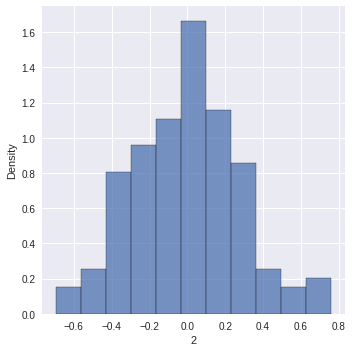
\includegraphics[width=\textwidth]{PC3_distribution.png}
         \caption{PC3}
     \end{subfigure}
        \caption{Distribution of PC features}
\end{figure}

The only thing we can say about these distributions is that they are centered. Now, let us see how much variance is explained depending on number of PC.
\begin{figure}[hbt!]
	\centering
	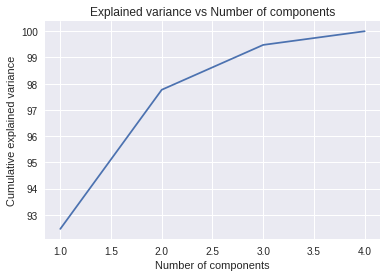
\includegraphics[width=0.7\textwidth]{explained_variance.png}
	\caption{Explained variance}
\end{figure}

If we use the first feature, it will explain 92\% of the data; if we use two features we are able to capture approximately 95\% of the data. If we use all features we are going to describe the entire dataset.

\exercise[{[Apply clustering algorithms]}]
The code implementation can be founded here \href{https://colab.research.google.com/drive/1x69gkP0C4YcYL_MKZ25hrghFE2HcYUKP?usp=sharing}{Code}.
In the first part we implement KMeans and EM algorithms on original DS and then we reduce dimension in order to visualize results.

\begin{figure}[hbt!]
     \centering
     \begin{subfigure}[b]{0.3\textwidth}
         \centering
         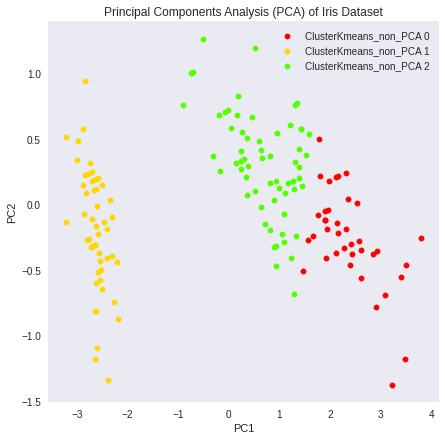
\includegraphics[width=\textwidth]{kmeans_non_pca.png}
         \caption{KMeans}
     \end{subfigure}
     \hfill
     \begin{subfigure}[b]{0.3\textwidth}
         \centering
         \includegraphics[width=\textwidth]{EM_non_pca.png}
         \caption{EM}
     \end{subfigure}
     \hfill
     \begin{subfigure}[b]{0.3\textwidth}
         \centering
         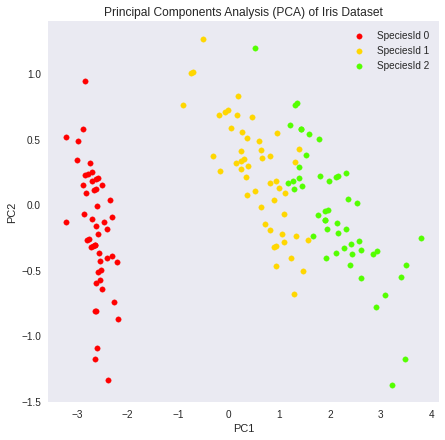
\includegraphics[width=\textwidth]{original_DS.png}
         \caption{Original}
     \end{subfigure}
        \caption{KMeans and EM clustering on original DS}
\end{figure}

In the second part we implement KMeans and EM algorithms on transformed DS via PCA with 2 components.

\begin{figure}[hbt!]
     \centering
     \begin{subfigure}[b]{0.3\textwidth}
         \centering
         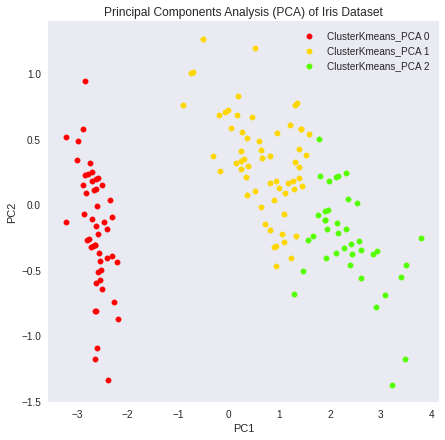
\includegraphics[width=\textwidth]{KMeans_PCA.png}
         \caption{KMeans}
     \end{subfigure}
     \hfill
     \begin{subfigure}[b]{0.3\textwidth}
         \centering
         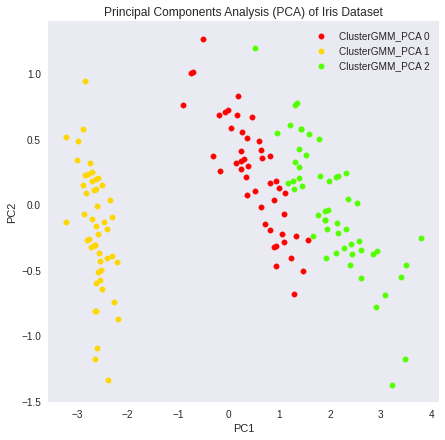
\includegraphics[width=\textwidth]{EM_PCA.png}
         \caption{EM}
     \end{subfigure}
     \hfill
     \begin{subfigure}[b]{0.3\textwidth}
         \centering
         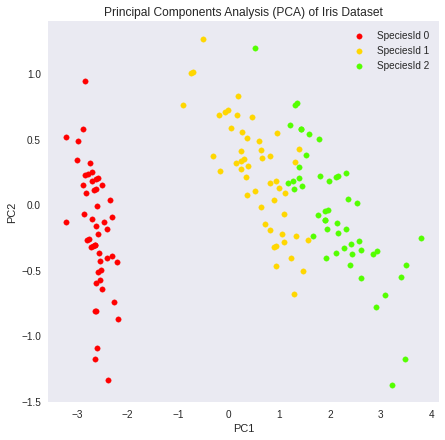
\includegraphics[width=\textwidth]{original_DS.png}
         \caption{Original}
     \end{subfigure}
        \caption{KMeans and EM clustering on transformed DS}
\end{figure}

Comparing results of EM and KMeans algoritms it is obvious that EM clustering performs better on the given DS. This is because, features are likely to be normally distributed. Hence, the EM clustering worked better at finding the actual species labels. Speaking about PCA implementation for clustering, in this case we use only 2 features, but the result remained approximately the same, since this 2 features explain 95\% of original data.
\end{document}